\documentclass[10pt,twocolumn]{scrartcl}

\usepackage[utf8]{inputenc}
\usepackage[T1]{fontenc}
\usepackage[ngerman]{babel}

\usepackage{amsmath}
\usepackage{amssymb}

\usepackage{graphicx}
\usepackage{tabularx}

\setlength{\parindent}{0cm}
\setlength{\parskip}{3mm}
\setlength{\textheight}{23.8cm}
\setlength{\headheight}{1cm}
\setlength{\topmargin}{-10mm}

\setlength{\oddsidemargin}{0cm}
\setlength{\evensidemargin}{0cm}
\setlength{\textwidth}{16cm}
\setlength{\columnsep}{8mm}

\usepackage{multicol}
\usepackage{colortbl}
\usepackage{xcolor}
\definecolor{grau}{gray}{0.95}
\definecolor{dunkelgrau}{gray}{0.85}

\usepackage[normal]{caption}

\setlength{\parindent}{5mm}
\setlength{\parskip}{0mm}

\usepackage{float}
\restylefloat{figure}

\renewcommand{\topfraction}{0.75}
\renewcommand{\textfraction}{0.2}

\newcommand{\TITLE}{Title Title Title Title}
\newcommand{\AUTHORS}{Lukas Rosenbach\\ David Lennart Risch}


%###########################################################
% die Sachen mit der Kopfzeile
\usepackage{lastpage}
\usepackage{fancyhdr}
\fancyhf{} % leere alle Felder
\fancyhead[R]{\footnotesize \AUTHORS}
\fancyhead[L]{\footnotesize \TITLE} % Titel des Aufsatzes
\fancyfoot[C]{\footnotesize \thepage/\pageref{LastPage}}
% \fancyfoot[C]{\footnotesize \thepage}
\renewcommand{\headrulewidth}{0.4pt} % obere Trennlinie
\pagestyle{fancy}
%###########################################################

\usepackage{listings}

\newcommand{\ownsection}[1]{\begin{center}\LARGE\textbf#1\end{center}}

\begin{document}

\twocolumn[
\ownsection{\TITLE}

\begin{center}
\AUTHORS \\
Mannheim, Juni 2020
\end{center}
\vspace*{5mm}
]

\section*{Abstract}

\section*{Einleitung}

\section*{Material und Methoden}

	\subsection*{Buffonsches Nadelproblem}
		Bei dem Buffonschen Nadelproblem, das erstmals von Buffon im Jahr 1733 behandelt wurde, geht es um die Wahrscheinlichkeit, dass eine Nadel, die auf eine Fläche mit parallelen Linien gleichen Abstands geworfen wird, eine Linie schneidet.
		
		Dieses Experiment beinhaltet eine Nadel der Länge l, die in einem Winkel $\theta$ auf eine Fläche mit parallelen Linien mit dem Abstand d fällt. Für eine kurze Nadel, also l < d, lässt sich die Wahrscheinlichkeit wie folgst berechnen: \cite{MathWorld}
		
		\begin{equation}
			x \equiv \frac{l}{d}
		\end{equation}
		
		\begin{align}
			P(x) &= \int_{0}^{2\pi}\frac{l|\cos{\theta}}{d}\frac{d\theta}{2\pi}\\ \nonumber
			&= \frac{2l}{\pi d}\int_{0}^{2\pi}\cos{\theta}d\theta\\ \nonumber
			&= \frac{2l}{\pi d}\\ \nonumber
			&= \frac{2x}{\pi} \nonumber
		\end{align}
		
		Für einen Linienabstand von 2l entspricht die Wahrscheinlichkeit $1/\pi$.
		
		\begin{align}
			P &= \frac{2l}{\pi d}\\ \nonumber
			&= \frac{2l}{\pi 2l}\\ \nonumber
			&= \pi \nonumber
		\end{align}
		
		Somit ist es möglich mithilfe eines Monte-Carlo-Verfahrens den Wert von Pi mit dem Buffonschen Nadelexperiment anzunähern.
	
	\subsection*{Implementierung des Experiments}
		Das Buffonsche Nadelproblem wurde als Python\cite{Python} Programm implementiert, um es mit einer großen Stichprobenzahl statistisch auswerten zu können. Außerdem enthält das Programm Funktionen für den Parameter- und Intervalltest.
		
		\subsubsection*{Die Simulation}
			Im ersten Schritt werden mehrere Nadelwürfe simuliert. Hier muss die Nadellänge, die Breite zwischen den Linien, die Anzahl der Linien und die Höhe des Feldes angegeben. Die Linien verlaufen in der Simulation vertikal. Rechts und links sind die Linien einen halben Linienabstand vom Rand des Feldes entfernt. So kann man gedanklich das Feld am rechten Rand wieder mit dem Linken Rand fortsetzen und erhält ein unendliches Feld. Dann wird für n Nadeln jeweils eine zufällige Position auf dem Feld und ein zufälliger Winkel berechnet. Diese Werte werden dann in einem Ergebnis gespeichert wo zusätzlich gezählt wird wie viele Nadeln eine Linie schneiden.
			
			\begin{figure}[htb]
				\centering
				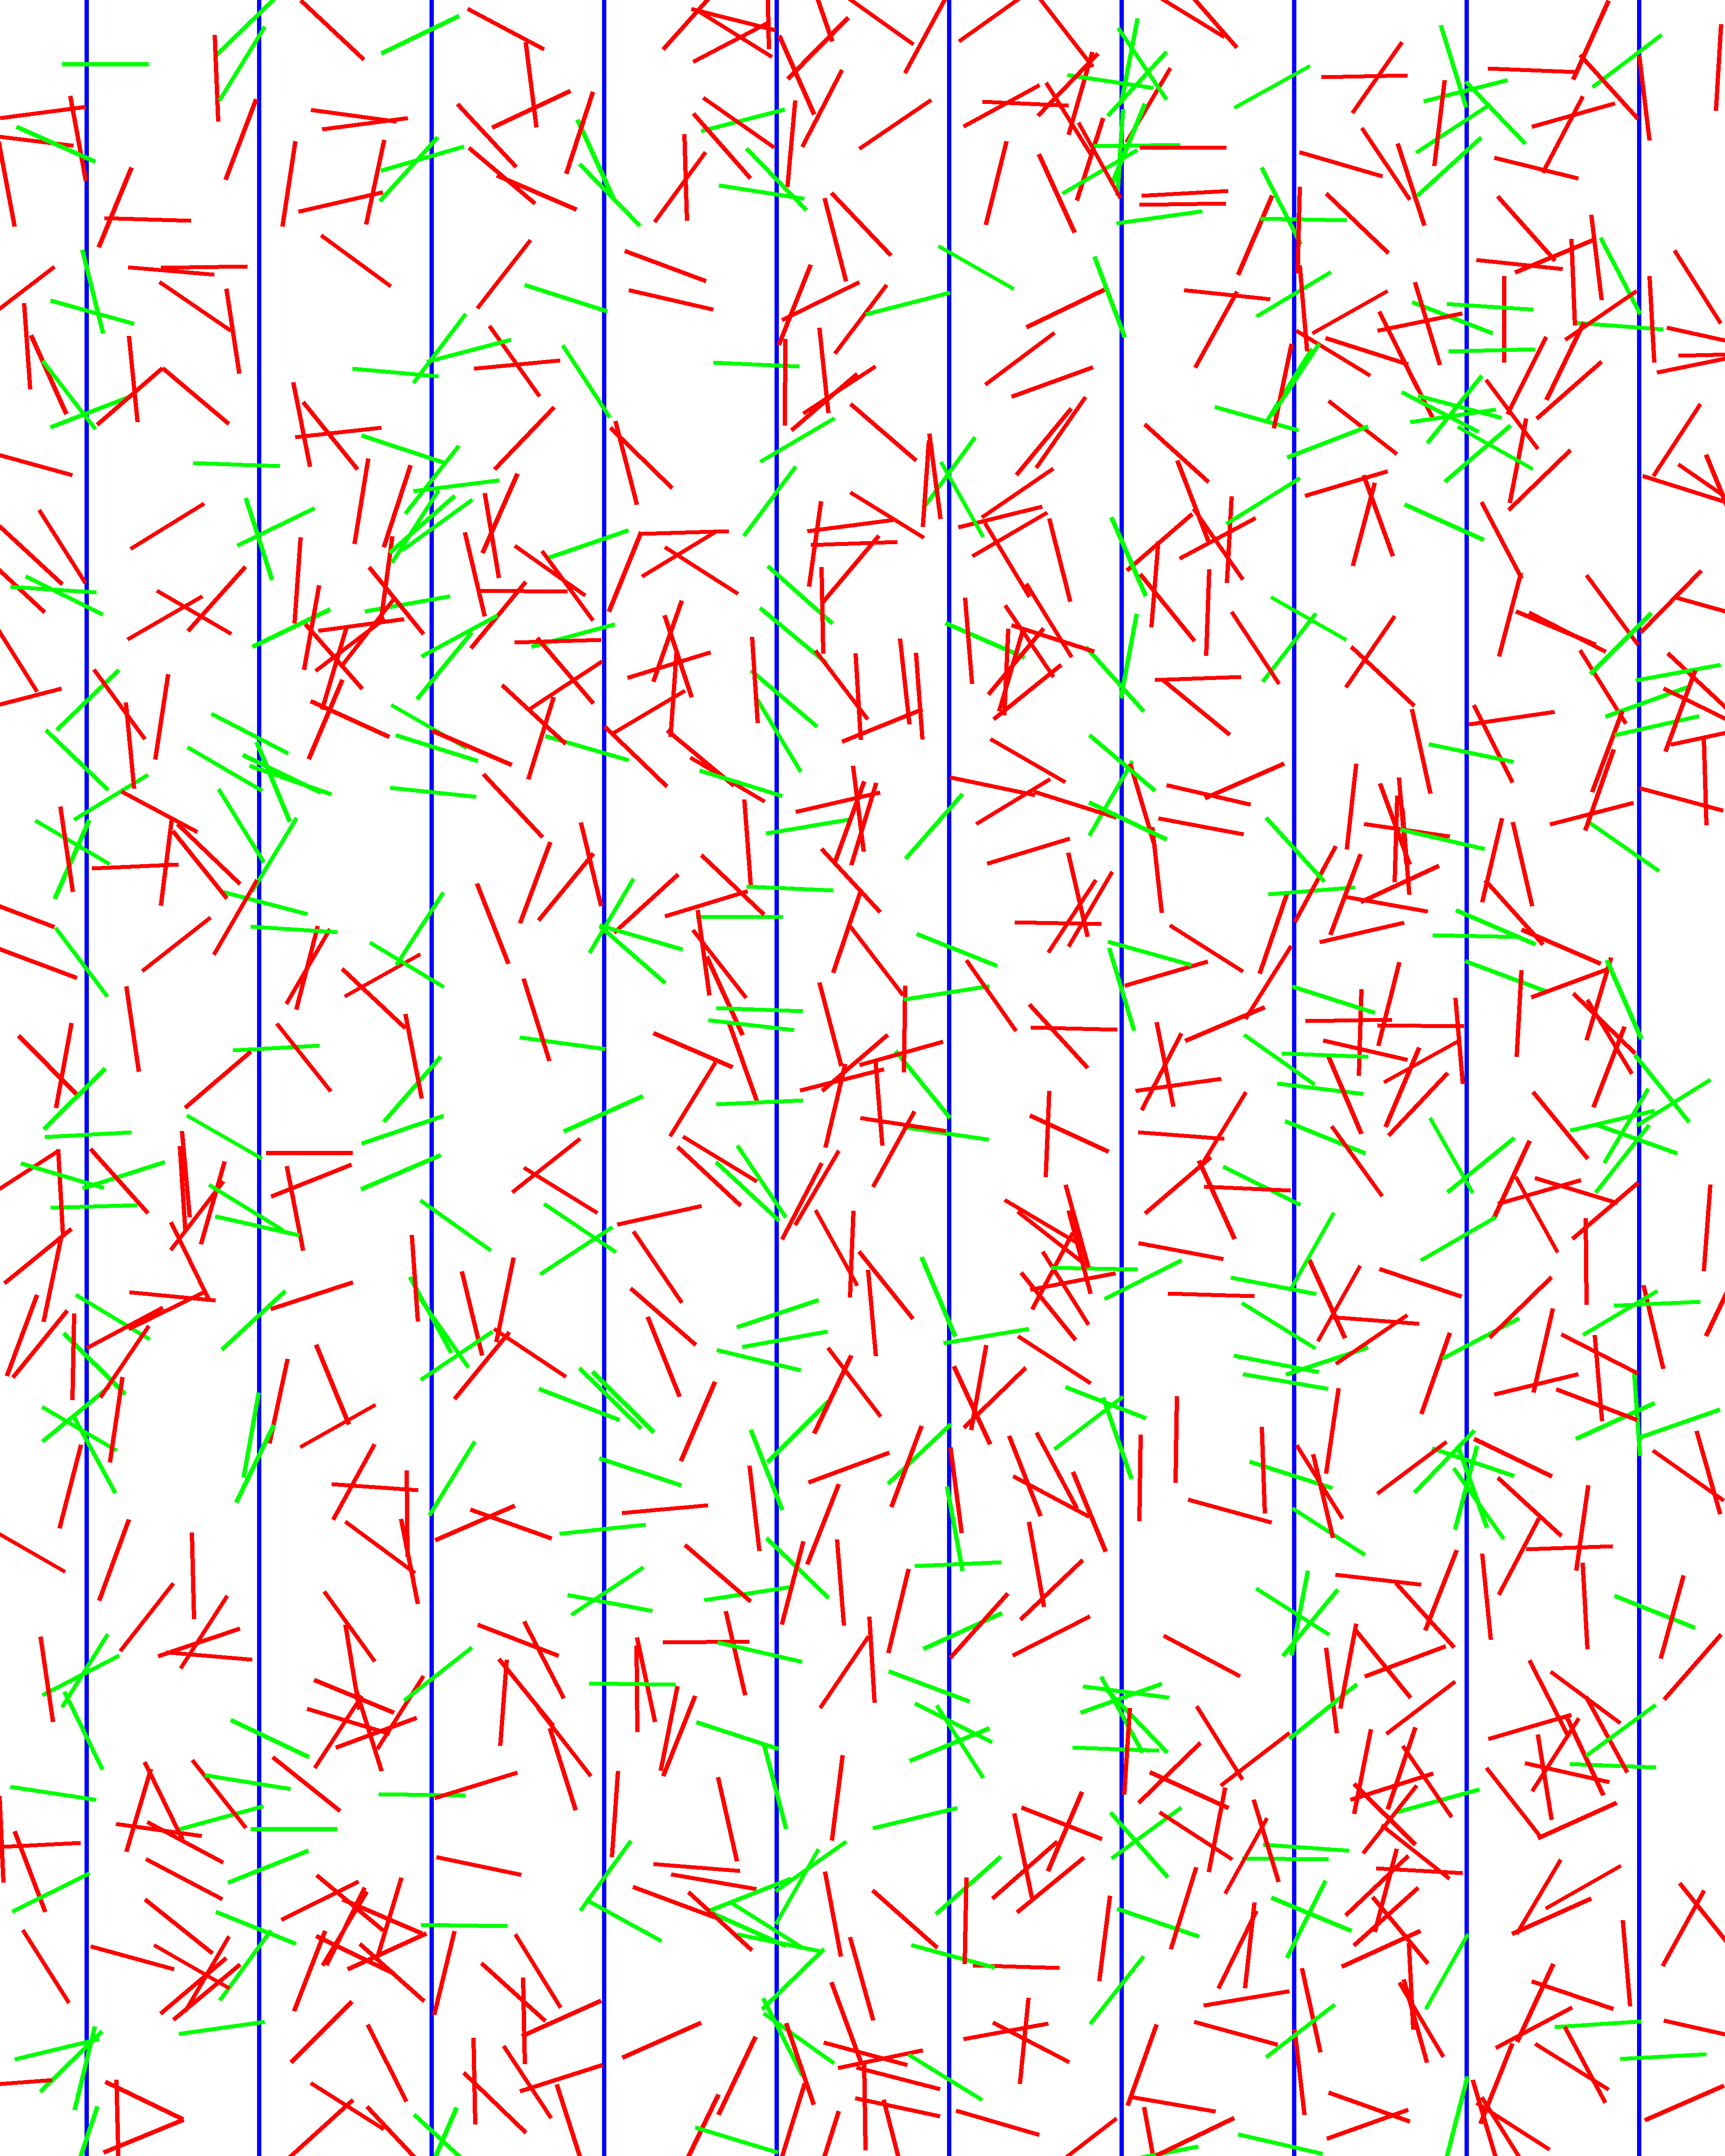
\includegraphics[width=0.45\textwidth]{img/needels.png}
				\caption{Ein Ergebnis der Simulation. Grüne Striche stellen Nadeln dar, die eine Linie schneiden. Rote Striche sind Nadeln, die keine Linie schneiden.}
				\label{fig:needels}
			\end{figure}
			
			Um zu prüfen, ob eine Nadel eine Linie schneidet wird der Abstand vom Mittelpunkt der Nadel zur nächsten Linie berechnet. Dann wird mit dem Winkel und der Nadellänge der Abstand in X-Richtung vom Mittelpunkt der Nadel zur Spitze berechnet. Wenn dieser Abstand größer als der Abstand zur nächsten Linie ist, schneidet die Nadel die Linie.
			Aus dem Ergebnis kann mit der Bibliothek Pillow\cite{Pillow} ein Bild (siehe Abbildung \ref{fig:needels}) erstellt werden, das die geworfenen Nadeln darstellt.

			Für die Statistische Auswertung enthält das Programm eine Methode, die Reihe von Simulationen durchführt. Für jede Simulation wird dabei die Anzahl der Nadeln, die eine Linie schneiden, in eine JSON-Datei geschrieben. Diese Datei enthält außerdem die Simulationsparameter, wie die Gesamtanzahl der Nadeln. Dies kann dann im nächsten Schritt ausgewertet werden.
		
		\subsubsection*{Die Auswertung}
			Es gibt verschiedene Möglichkeiten die Simulationen mit dem Programm auszuwerten. Als erstes kann man aus der JSON-Datei ein Histogramm erzeugen, das die Häufigkeit eines Ergebnisses darstellt. Erstellt werden die Diagramme mit der Bibliothek matplotlib\cite{matplotlib}. Ein Ergebnis ist die Anzahl der Nadeln, die eine Linie schneiden. In Abbildung \ref{fig:hist} sieht man, dass die Ergebnisse normalverteilt sind.
			
			\begin{figure}[htb]
				\centering
				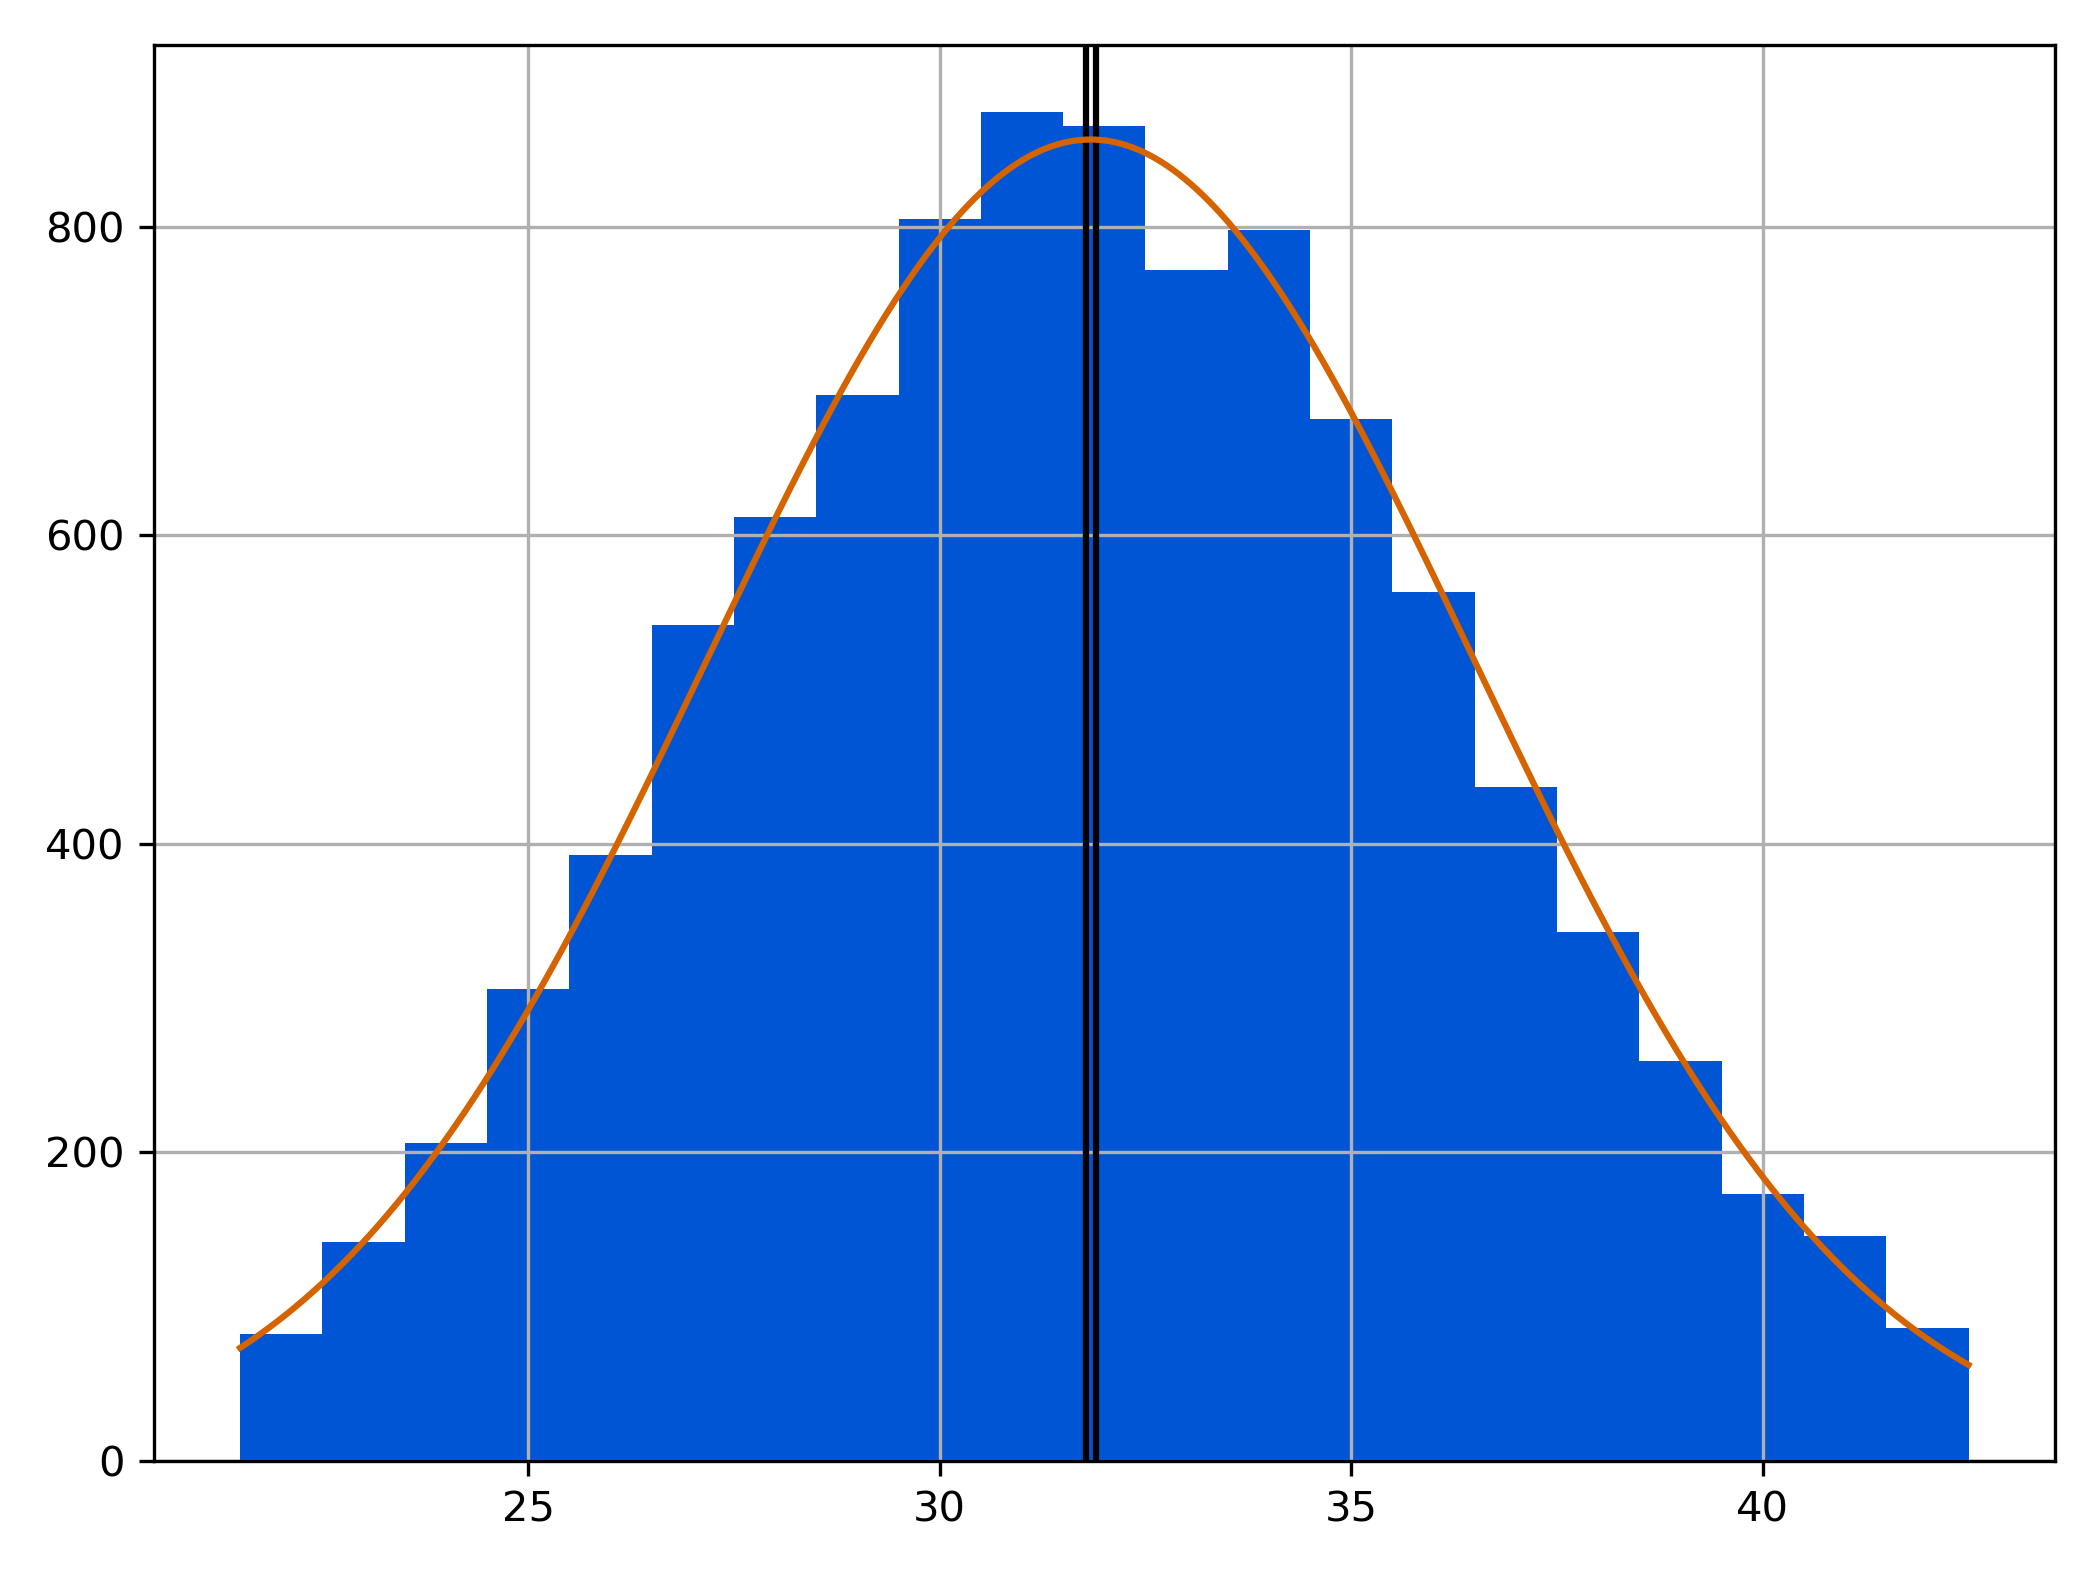
\includegraphics[width=0.45\textwidth]{img/histogram_10000.png}
				\caption{Histogramm von 10000 Simulationen mit 100 Nadeln}
				\label{fig:hist}
			\end{figure}
		
			Außerdem lässt sich ein Parameter- und Intervalltest anwenden, die im folgenden Kapitel beschrieben werden.
		
\section*{Durchführung}

\section*{Ergebnisse und Diskussion}

\begin{thebibliography}{99}
	\bibitem{MathWorld}Weisstein, Eric W.: {\it Buffon's Needle Problem.}, From MathWorld--A Wolfram Web Resource. https://mathworld.wolfram.com/BuffonsNeedleProblem.html
	\bibitem{Python}Python: https://www.python.org/
	\bibitem{Pillow}Pillow: https://pillow.readthedocs.io/en/stable/
	\bibitem{matplotlib}matplotlib: https://matplotlib.org/
\end{thebibliography}

\end{document}